\chapter{Medición del espesor de la \glsentrytext{coroides}}
\section{Problema}
Los estudios demuestran que hay una relación entre el grosor de la
\emph{\gls{coroides}} y la aparición de la \emph{\gls{uveitis}}. Es
necesario, por tanto, medir el espesor de la \emph{\gls{coroides}}
para valorar el impacto de esta enfermedad y para seguir su evolución
en el tiempo.\\
La \emph{\gls{coroides}} o \emph{úvea} es una membrana por la que
pasan gran cantidad de vasos sanguíneos, cuya función es mantener la
temperatura
constante y nutrir ciertas estructuras del globo ocular. \\
Gracias a las \gls{tco} es posible medir el grosor de la membrana. Sin
embargo, el software de la máquina no realiza la medición de forma
automática, sino que es necesario trazar la línea a mano. Esto
ralentiza el proceso y, además, genera imprecisiones en las mediciones
debidos principalmente a fallos humanos: Si la imagen no está en
posición horizontal es difícil trazar una línea perpendicular, puede
fallar el pulso, etc. Esta línea se debe trazar por el punto de menor
grosor de la retina, conocido como \emph{\gls{fovea}} y de forma
perpendicular a la \emph{\gls{mBruch}}. Una vez trazada la línea, hay
que medirla.


\section{Objetivos}
Los objetivos puestos en común después de sucesivas reuniones fueron:
\begin{itemize}
\item Automatizar lo máximo posible o requerir intervención mínima del
  oftalmólogo en el proceso de marcado de los puntos del espesor a
  medir de la \emph{\gls{coroides}}.
\item Una vez delimitado el espesor de la \emph{\gls{coroides}},
  proporcionar su medida en micras lo más fielmente posible.
\end{itemize}
Cumplir estos objetivos propuestos proporcionaría al estudio de la
evolución y control de la \emph{\gls{uveitis}} una automatización
completa del seguimiento, pudiendo realizar las medidas de todo el
historial de un paciente en pocos segundos. Lo más importante no es el
tiempo ahorrado sino la erradicación de errores de precisión manuales
y resultados distintos de una misma imagen.

\section{Estudio}
El estudio se ha realizado en distintas fases, todas ellas de manera
secuencial y acumulativa. Además de la documentación de cada fase, se
proporcionan las mismas imágenes de guía y apoyo usadas durante el
estudio.  Sin embargo, aunque las fases aquí expuestas se encuentren
en orden secuencial, el orden cronológico en el que se resolvieron
varía, debido a que con cada nueva imagen que se estudiaba surgían
nuevos problemas.
\begin{enumerate}
\item El primer paso consistió en \textbf{extraer} de la imagen
  original \textbf{el área de interés}. Las máquinas \gls{tco} siempre
  proporcionan, además
  de la zona de estudio, el corte usado sobre la estructura ocular. \\
  \textbf{Se desarrolló una biblioteca encargada de automatizar la
    extracción del área de estudio.}
\item El corte programado durante la exploración tiene un grado de
  inclinación sobre la estructura ocular. \textbf{En la mayoría de las
    exploraciones el corte no es horizontal}, si se realizan
  exploraciones desde todos los ángulos, sólo uno muestra la
  estructura
  de manera horizontal. \\
  \textbf{Se desarrolló un algoritmo para la corrección de la
    inclinación} y así rotar la imagen el grado de desviación del
  corte con respecto a la horizontal de la estructura ocular.
\item Corregida la inclinación de la estructura y para poder realizar
  la medición de la \emph{\gls{coroides}}, \textbf{es necesario}
  previamente
  \textbf{establecer un punto de referencia, la \emph{\gls{fovea}}}. \\
  \textbf{Se desarrolló un algoritmo para la detección del punto con
    el menor grosor de la retina, la \emph{\gls{fovea}}.}
\item Una vez fijada la \emph{\gls{fovea}} \textbf{se marcan los dos
    puntos
    de la \emph{\gls{coroides}} necesarios para poder medir su espesor}. \\
  \textbf{Se desarrolló un algoritmo para la detección de los puntos
    de espesor de la \emph{\gls{coroides}}}
\item Finalmente, \textbf{se realiza la medición del espesor de la
    \emph{\gls{coroides}}}. Este es el proceso más delicado e
  impreciso de todo el estudio porque al aplicar tantas técnicas de
  procesamiento a la imagen de manera consecutiva, hay que dar una
  medida en micras con el mínimo error de precisión posible del
  espesor de la \emph{\gls{coroides}}. \\
  \textbf{Se desarrolló un algoritmo para la medición en micras del
    espesor de la \emph{\gls{coroides}}}
\end{enumerate}

\section{Algoritmo propuesto}
\begin{enumerate}
\item La primera fase consistió en delimitar y extraer el
  área\deftecnica{tecnica:roi} a investigar. Esto es así, porque las
  máquinas \gls{tco} en una misma
  imagen presentan el corte analizado y su resultado.\\
  Para resolver este problema de forma automática se procedió a
  realizar una biblioteca que realiza el siguiente procedimiento a la
  imagen.
  \begin{enumerate}[label*=\arabic*.]
  \item Convierte la imagen de escala \emph{RGB} a \emph{escala de
      grises\deftecnica{tecnica:cambio-color}}.

    \begin{figure}[H]
      \caption{Original}
      \centering \setlength\fboxsep{0pt} \setlength\fboxrule{0.5pt}
      \fbox{\includegraphics[width=\textwidth]{imagenes/espesor_coroides/AlgoritmoOriginal.png}}
    \end{figure}

  \item Duplica la imagen, en una aplica un \emph{threshold
      Otsu\deftecnica{tecnica:threshold-otsu}} con
    \emph{dilation\deftecnica{tecnica:dilation}} y en otra un
    \emph{threshold binario\deftecnica{tecnica:threshold-binario}}
    para \emph{binarizar} la imagen.
 
    \begin{figure}[H]
      \caption{Duplicado Threshold Otsu}
      \centering \setlength\fboxsep{0pt} \setlength\fboxrule{0.5pt}
      \fbox{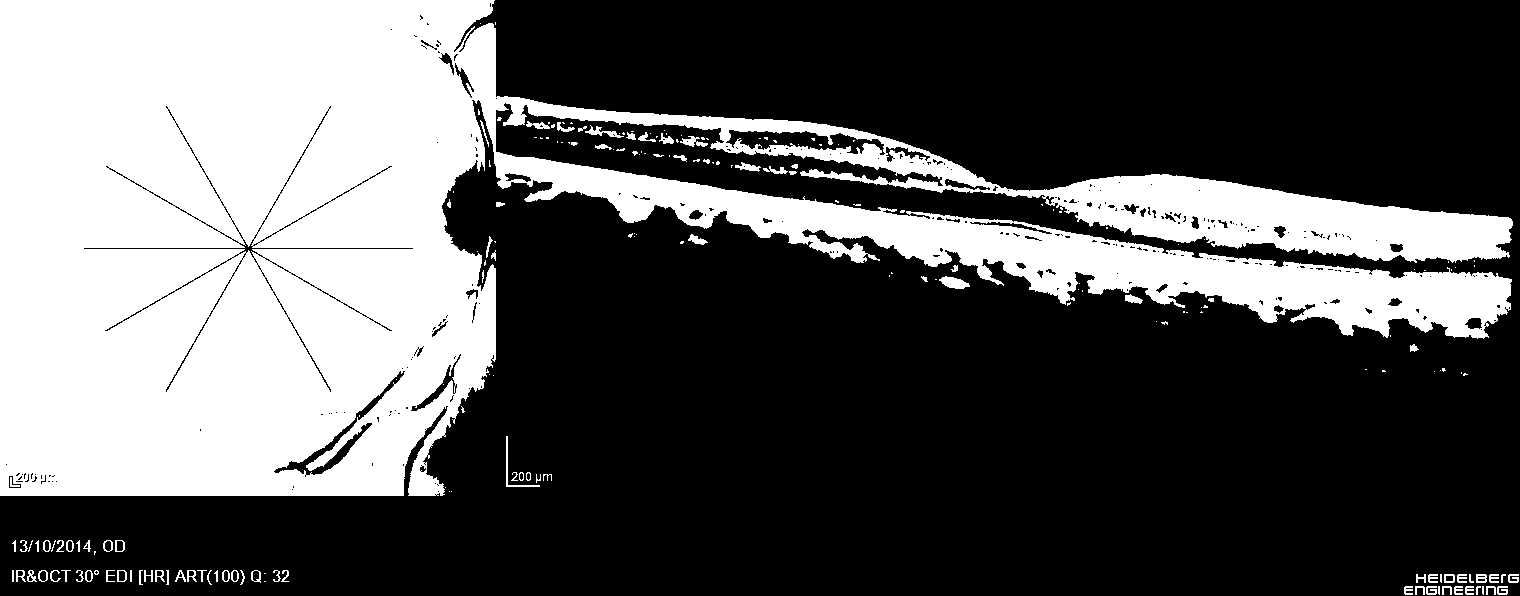
\includegraphics[width=\textwidth]{imagenes/espesor_coroides/Algoritmo_2_roi_otsu_first_point.png}}
    \end{figure}

    \begin{figure}[H]
      \caption{Duplicado Threshold Otsu con Dilation}
      \centering \setlength\fboxsep{0pt} \setlength\fboxrule{0.5pt}
      \fbox{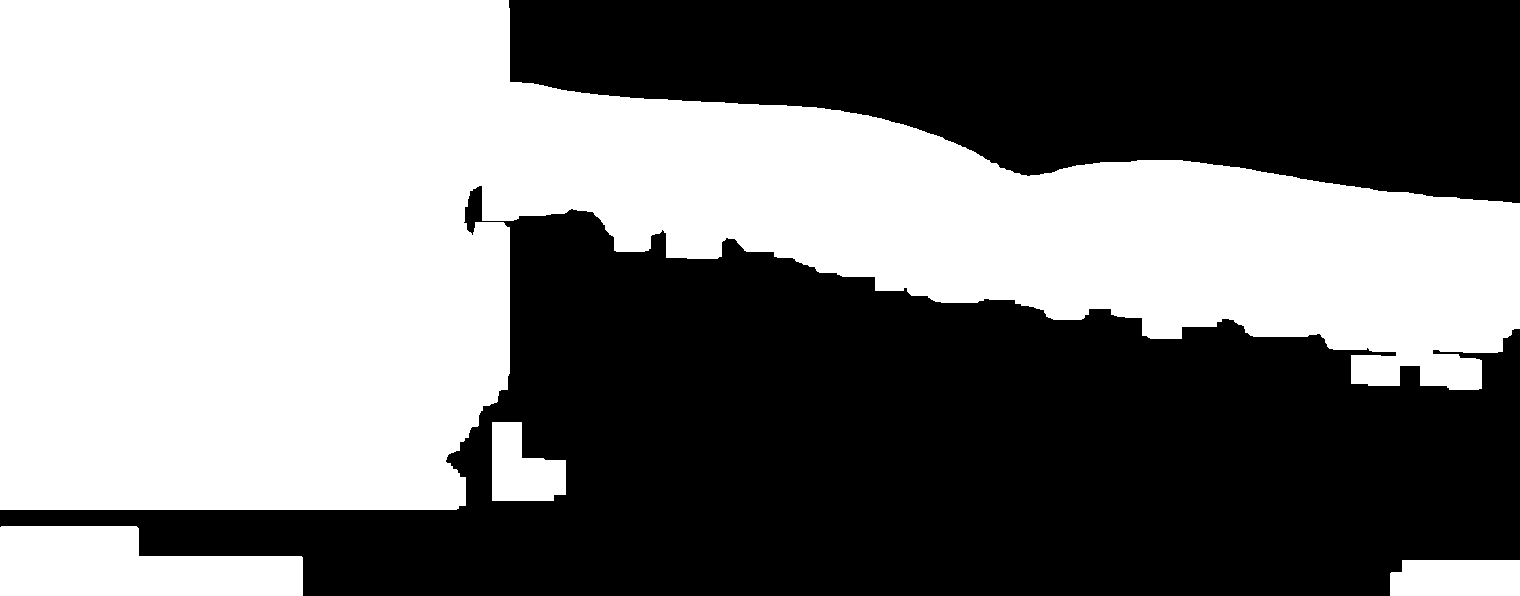
\includegraphics[width=\textwidth]{imagenes/espesor_coroides/Algoritmo_3_roi_otsu_dilation.png}}
    \end{figure}

  \item Se recorre la imagen del \emph{threshold Otsu} con una
    horizontal de derecha a izquierda, desde la esquina superior
    derecha con las coordenadas, $0$ como $x$ y ancho de la imagen
    como $y$ encontrar el borde de separación entre las dos imágenes.
    Este borde está ligeramente desplazado a la derecha para ignorar
    espacios en negro.

    \begin{figure}[H]
      \caption{Primer punto de separación}
      \centering \setlength\fboxsep{0pt} \setlength\fboxrule{0.5pt}
      \fbox{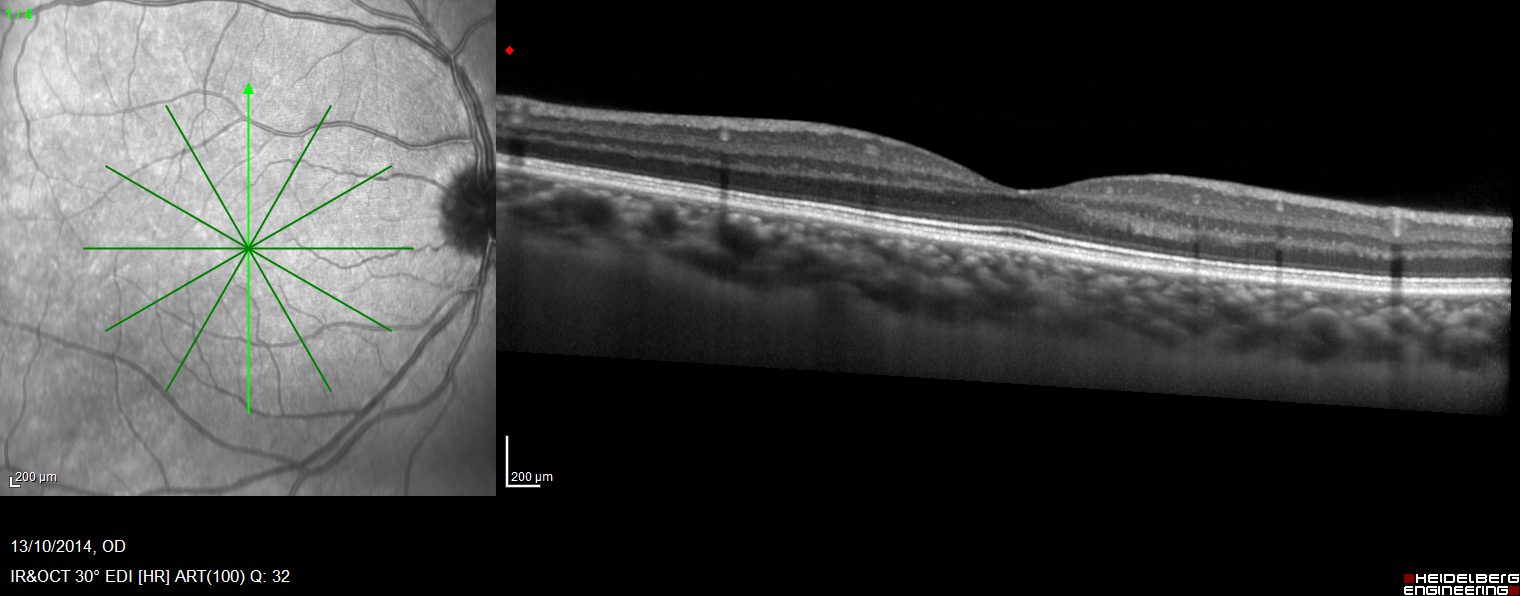
\includegraphics[width=\textwidth]{imagenes/espesor_coroides/Algoritmo_4_roi_first_point.png}}
    \end{figure}

  \item Al conocer el \textbf{punto del borde de separación en la
      parte superior}, queda buscarlo también en la parte inferior de
    abajo a arriba en la imagen del \emph{threshold binario} con las
    coordenadas, el borde de separación como $x$ y la altura de la
    imagen como $y$.

    \begin{figure}[H]
      \caption{Duplicado Threshold Binario}
      \centering \setlength\fboxsep{0pt} \setlength\fboxrule{0.5pt}
      \fbox{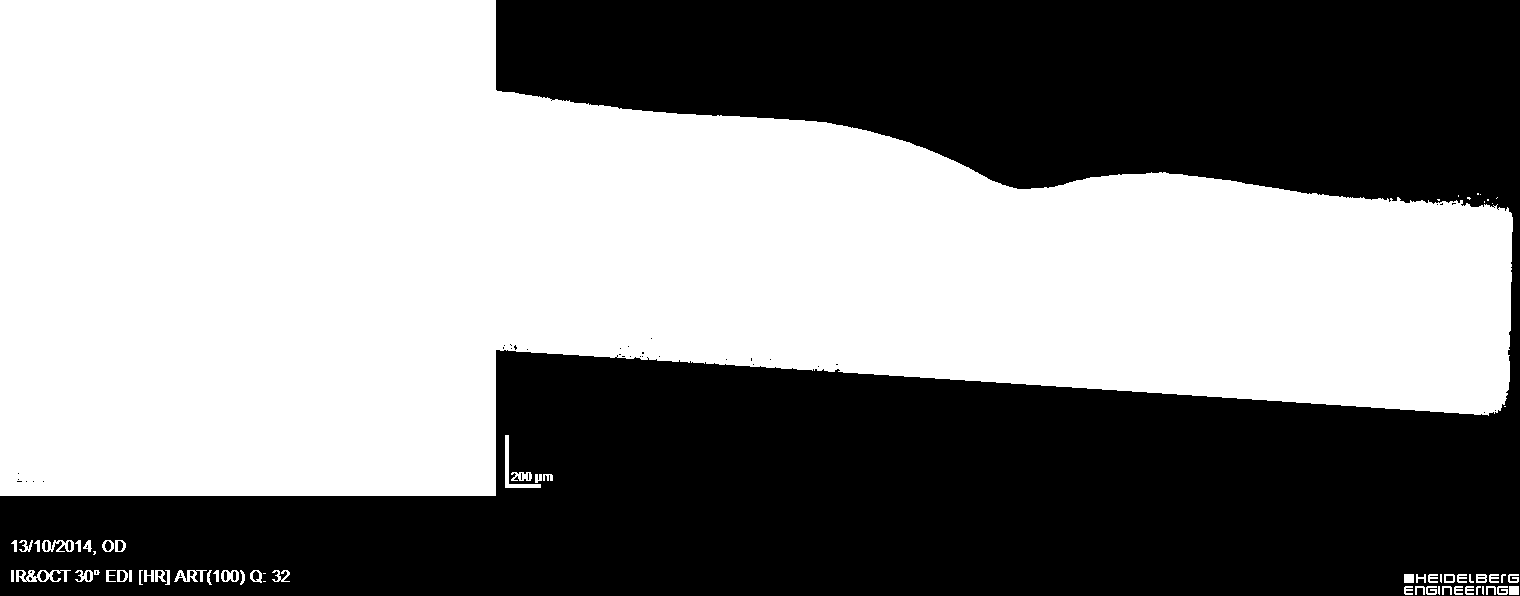
\includegraphics[width=\textwidth]{imagenes/espesor_coroides/Algoritmo_5_roi_binary_first_point.png}}
    \end{figure}

    \begin{figure}[H]
      \caption{Segundo punto de separación}
      \centering \setlength\fboxsep{0pt} \setlength\fboxrule{0.5pt}
      \fbox{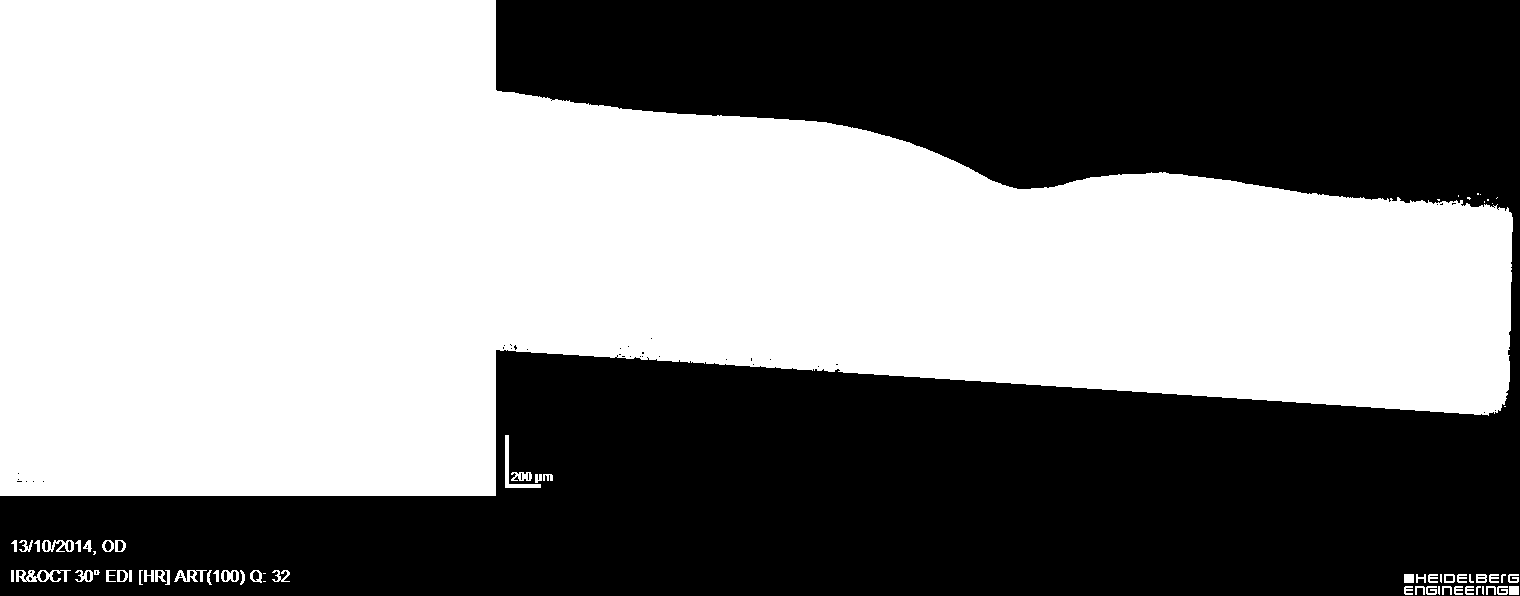
\includegraphics[width=\textwidth]{imagenes/espesor_coroides/Algoritmo_5_roi_binary_first_point.png}}
    \end{figure}

  \item Con estos puntos ya se puede obtener la zona de la imagen
    original a estudiar. \textbf{Si se apura y se recorta el negro
      sobrante de la parte inferior evita errores} en la detección del
    segundo punto de la \emph{\gls{coroides}} en algunos casos.

    \begin{figure}[H]
      \caption{Parte inferior a borrar}
      \centering \setlength\fboxsep{0pt} \setlength\fboxrule{0.5pt}
      \fbox{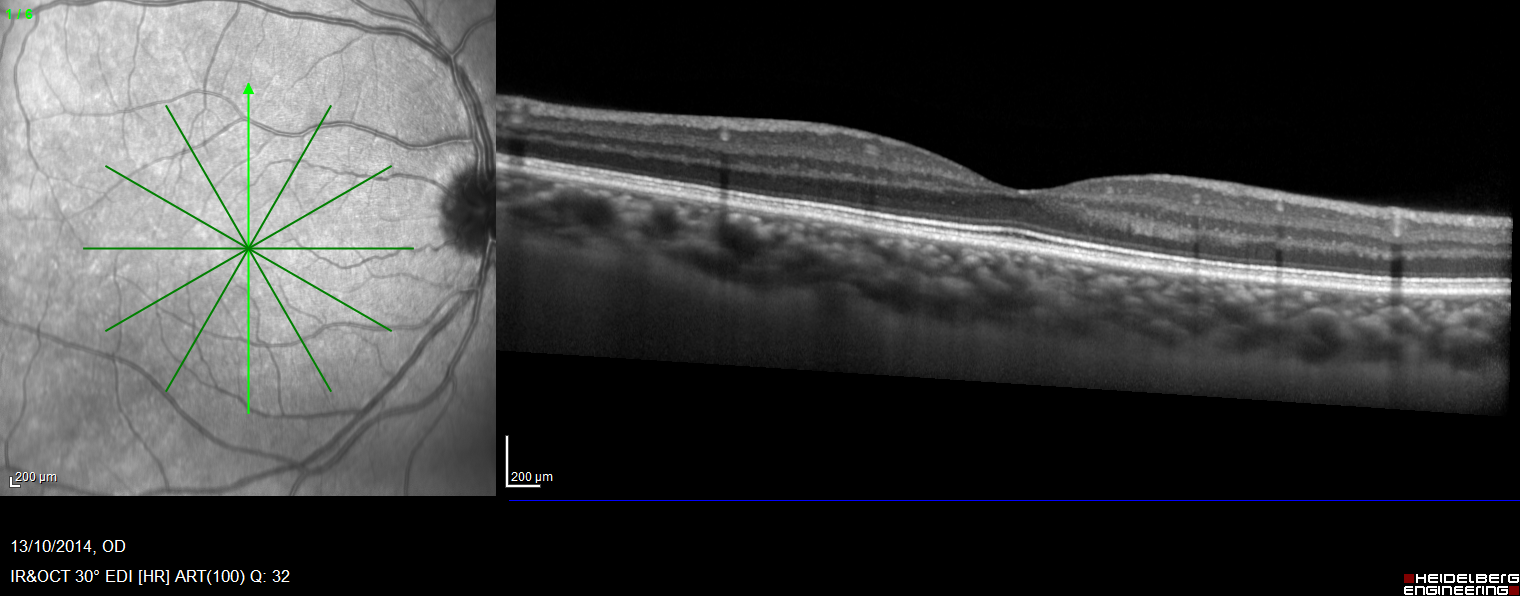
\includegraphics[width=\textwidth]{imagenes/espesor_coroides/Algoritmo_7_roi_botton_lower_line.png}}
    \end{figure}

    \begin{enumerate}[label*=\arabic*.]
    \item \textbf{Para eliminar dicha zona} y como la imagen no tiene
      por qué estar en posición horizontal, \textbf{se procede a
        buscar dos puntos auxiliares}: uno empieza con la $x$ igual a
      $2/4$ de la anchura de la imagen, y el otro con la $x$ igual a
      $3/4$ de la anchura. Ambos empiezan con $y$ igual al borde
      inferior provisional hacia arriba, ignorando toda el área negra.

      \begin{figure}[H]
        \caption{Puntos auxiliares}
        \centering \setlength\fboxsep{0pt} \setlength\fboxrule{0.5pt}
        \fbox{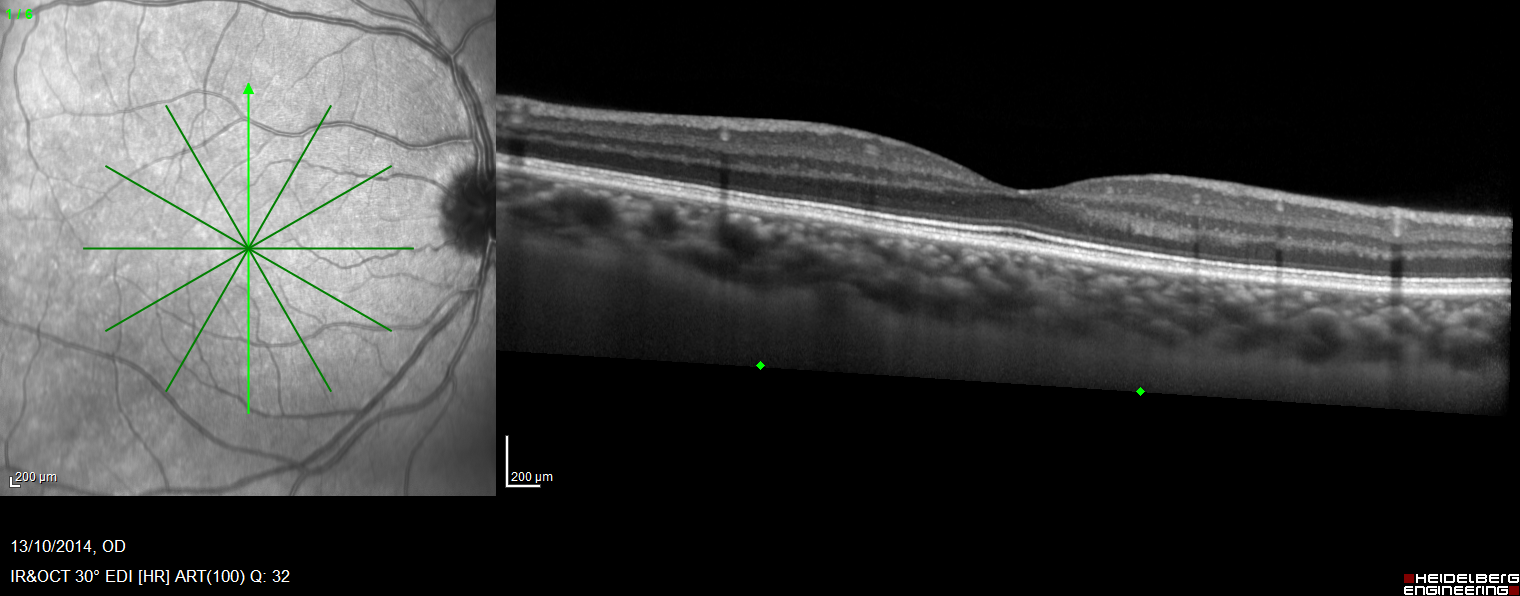
\includegraphics[width=\textwidth]{imagenes/espesor_coroides/Algoritmo_10_roi_aux_middle_points.png}}
      \end{figure}

    \item \textbf{Una vez obtenidos los dos puntos, se procede a
        obtener el punto definitivo para generar el rectángulo} que
      contiene la imagen de estudio.

    \item \textbf{Para calcular dicho punto}, el que está situado más
      cerca del borde inferior para no recortar parte de la propia
      imagen si no está horizontal, \textbf{hay que calcular primero}
      otros dos. Esos puntos son \textbf{la intersección con el borde
        de sepación y de una recta imaginaria con los puntos
        auxiliares} del paso anterior. Se calculan añadiendo a la $y$
      de cada punto auxiliar la diferencia con respecto a la $y$ del
      otro punto auxiliar.

      \begin{figure}[H]
        \caption{Puntos de intersección (en rojo) y auxiliares
          (verde)}
        \centering \setlength\fboxsep{0pt} \setlength\fboxrule{0.5pt}
        \fbox{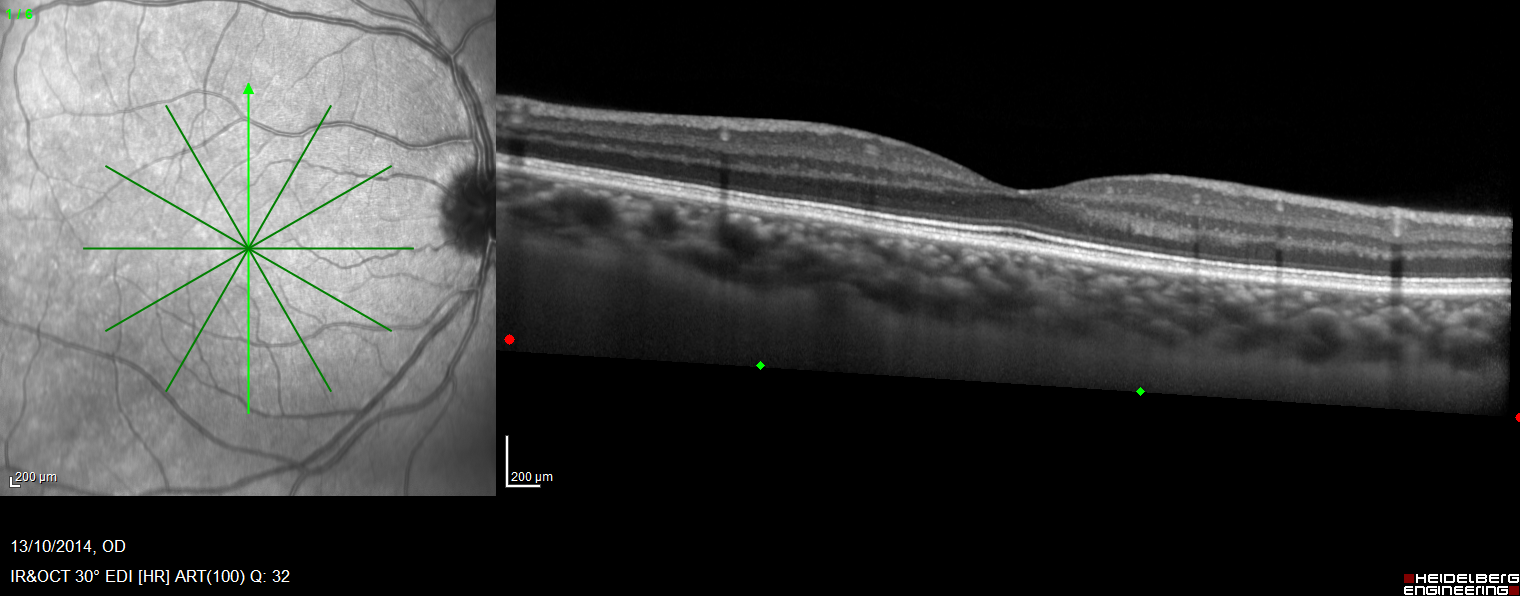
\includegraphics[width=\textwidth]{imagenes/espesor_coroides/Algoritmo_14_roi_all_points.png}}
      \end{figure}

    \item Obtenidos estos dos puntos, el que tenga mayor $y$, es el
      más cercano al borde inferior y por tanto el utilizado como base
      para obtener el segundo punto del rectángulo.

      \begin{figure}[H]
        \caption{Segundo punto del rectángulo}
        \centering \setlength\fboxsep{0pt} \setlength\fboxrule{0.5pt}
        \fbox{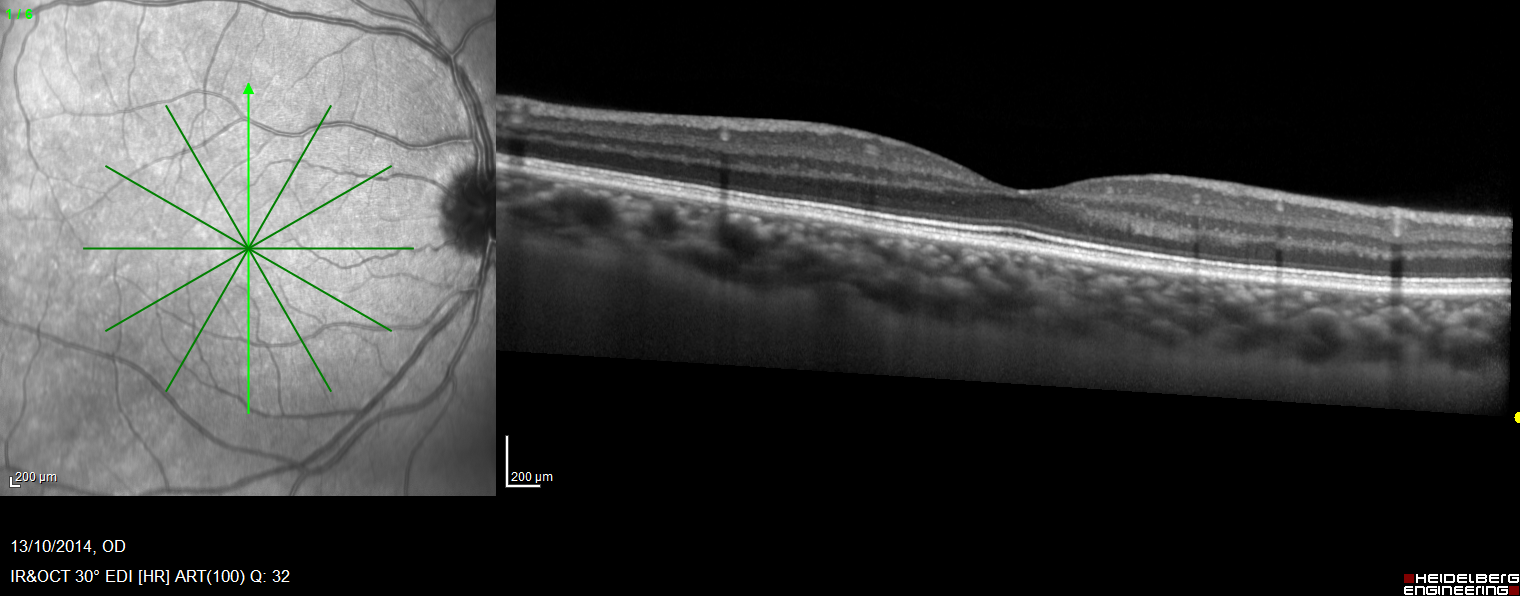
\includegraphics[width=\textwidth]{imagenes/espesor_coroides/Algoritmo_15_roi_final_point.png}}
      \end{figure}

    \item Finalmente, \textbf{se obtiene el rectángulo que contiene a}
      la parte de \textbf{la imagen} que queremos estudiar \textbf{con
        el punto del borde de separación de la parte superior y el
        punto} formado por la $y$ del punto \textbf{más cercano al
        borde inferior} del paso anterior y la anchura de la imagen
      original como la $x$.

      \begin{figure}[H]
        \caption{Zona de interés o \emph{ROI}}
        \centering \setlength\fboxsep{0pt} \setlength\fboxrule{0.5pt}
        \fbox{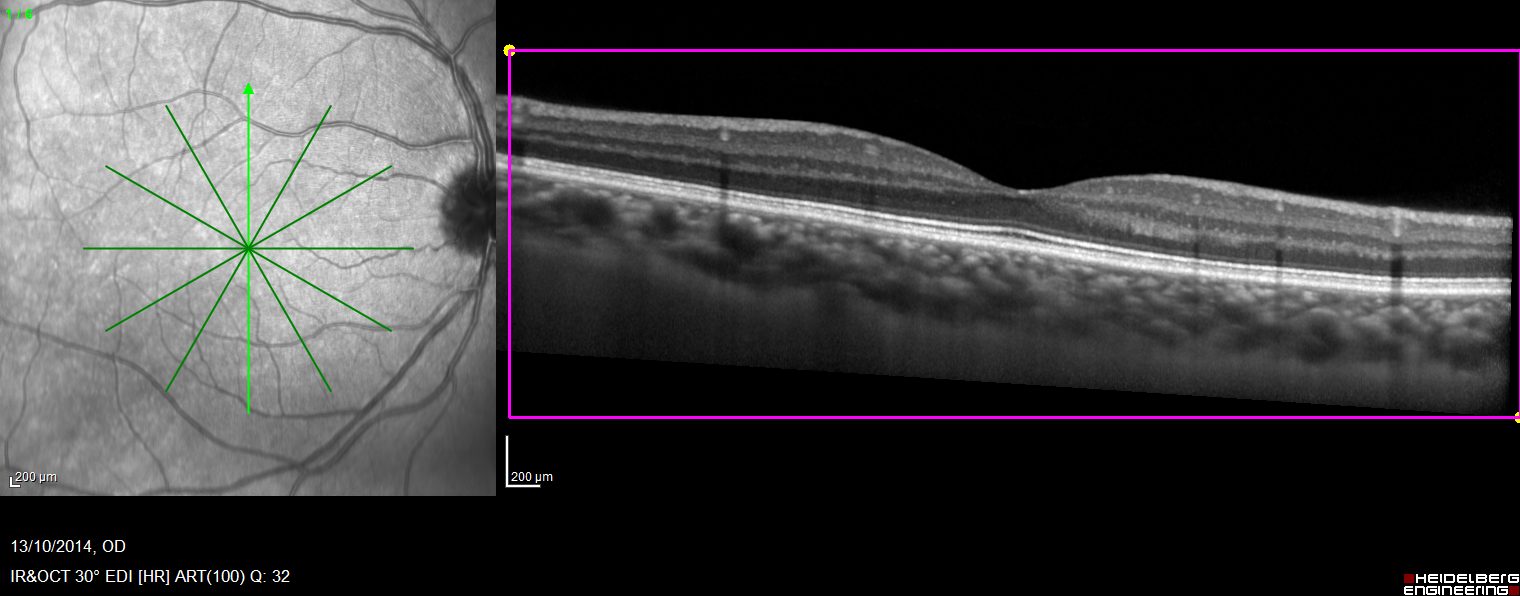
\includegraphics[width=\textwidth]{imagenes/espesor_coroides/Algoritmo_17_roi_final_rectangle.png}}
      \end{figure}

    \end{enumerate}
  \end{enumerate}
\item Una vez delimitada la zona de interés, \textbf{es necesario
    corregir la inclinación del corte de la máquina} con respecto de
  la estructura ocular. \\
  Para esta labor se desarrolló una biblioteca, que aplica el
  siguiente procedimiento a la imagen.
  \begin{enumerate}[label*=\arabic*.]
  \item \textbf{El primer paso mide el ángulo de inclinación} de la
    estructura ocular \textbf{para así poder realizar la rotación que
      la corrija}.  Para ello se busca y escoge un ángulo de
    referencia, aplicando la \emph{Transformada de
      Hough\deftecnica{tecnica:hough}} para rectas. La estructura
    ocular posee una capa con una intensidad muy alta denominada
    \emph{\gls{mBruch}} en la que si se aplica dicha transformada, se
    obtiene sobre ella una recta que puede ser usada como
    referencia. Todas las líneas detectadas están almacenadas de forma
    paramétrica en una matriz de pares $\left(\rho, \theta \right)$.
    La primera línea de la matriz que no sea vertical
    ($\theta \neq 0º$) es la recta buscada sobre la membrana. Para aplicar
    esta técnica es necesario aplicar primero un filtro para detectar
    los bordes:

      \begin{figure}[H]
        \caption{Canny para aplicar Transformada de Hough}
        \centering \setlength\fboxsep{0pt} \setlength\fboxrule{0.5pt}
        \fbox{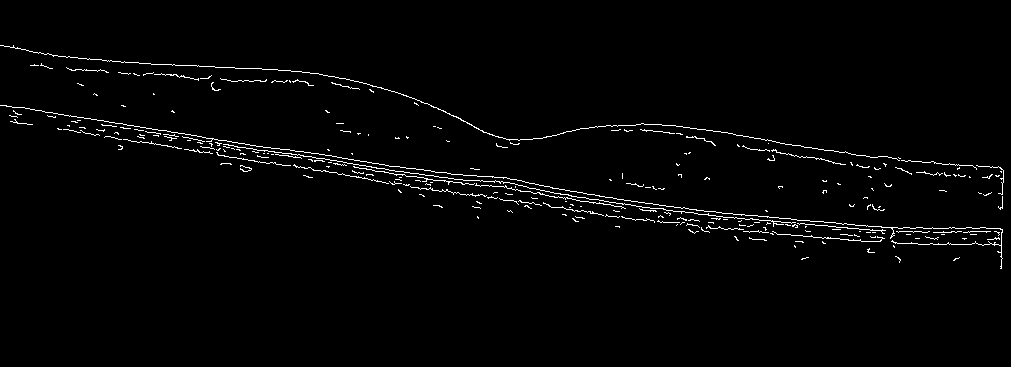
\includegraphics[width=\textwidth]{imagenes/espesor_coroides/Algoritmo_18_horizontal_Canny_Hough.png}}
      \end{figure}

      \begin{figure}[H]
        \caption{Línea detectada}
        \centering \setlength\fboxsep{0pt} \setlength\fboxrule{0.5pt}
        \fbox{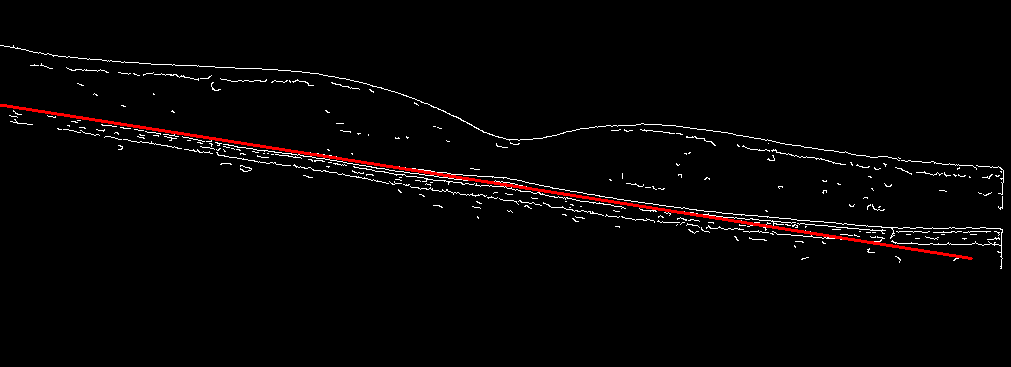
\includegraphics[width=\textwidth]{imagenes/espesor_coroides/Algoritmo_19_horizontal_Canny_Hough_recta.png}}
      \end{figure}


  \item \textbf{Una vez obtenida la $\theta$ de la pendiente a corregir
      respecto la horizontal} $\left( \theta = 90º \right)$ hay que
    calcular la diferencia de inclinación. Para ello se calcula la
    diferencia con la siguiente fórmula:
    \begin{equation*}
      \theta_\text{Corrección} = \theta_{Bruch} - \theta_{horizontal}
    \end{equation*}
    \begin{center}
      siendo $\theta_{horizontal} = 90º$
    \end{center}
  \item \textbf{Finalmente} se procede a \textbf{rotar la imagen} con
    la $\theta_{\text{Corrección}}$, usando como centro de rotación el
    punto central de la imagen.

      \begin{figure}[H]
        \caption{Imagen rotada}
        \centering \setlength\fboxsep{0pt} \setlength\fboxrule{0.5pt}
        \fbox{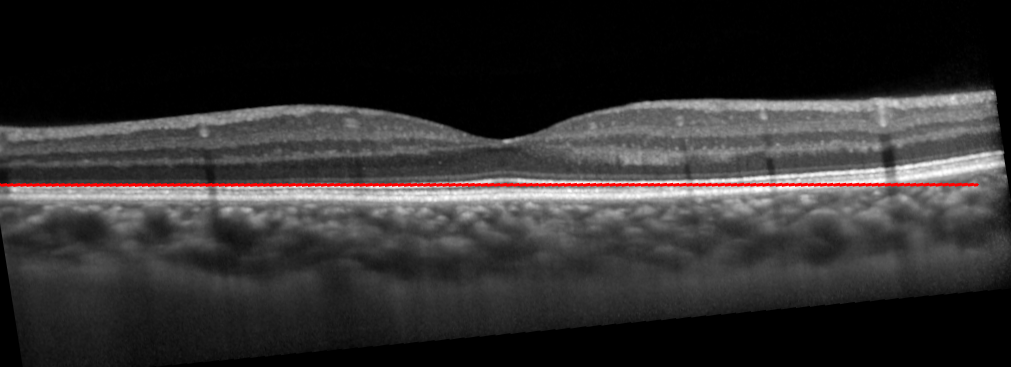
\includegraphics[width=\textwidth]{imagenes/espesor_coroides/Algoritmo_22_horizontal_Horizontal_recta.png}}
      \end{figure}

  \end{enumerate}

\item Teniendo la imagen horizontal para evitar fallos debidos a la
  inclinación, se procedió a desarrollar un algoritmo para
  \textbf{encontrar el punto de referencia, la \emph{\gls{fovea}}}.
  \begin{enumerate}[label*=\arabic*.]
  \item \textbf{Se somete} una copia de \textbf{la imagen} (para no
    alterar la original) \textbf{a un \emph{median
        Blur\deftecnica{tecnica:blur-median}}} con un \emph{kernel} de
    tamaño $7$ \textbf{para eliminar el ruido granulado}.

      \begin{figure}[H]
        \caption{Resultado del Blur}
        \centering \setlength\fboxsep{0pt} \setlength\fboxrule{0.5pt}
        \fbox{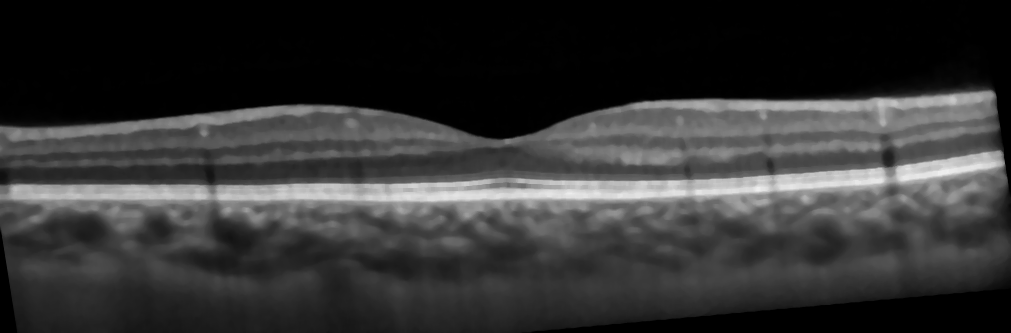
\includegraphics[width=\textwidth]{imagenes/espesor_coroides/Algoritmo_26_fovea_blur.png}}
      \end{figure}

  \item Sobre esta copia transformada, \textbf{se aplica un
      \emph{threshold binario}} con valor umbral de $30$. Con esto se
    pretende binarizar la imagen para facilitar el siguiente paso.

      \begin{figure}[H]
        \caption{Resultado del Threshold}
        \centering \setlength\fboxsep{0pt} \setlength\fboxrule{0.5pt}
        \fbox{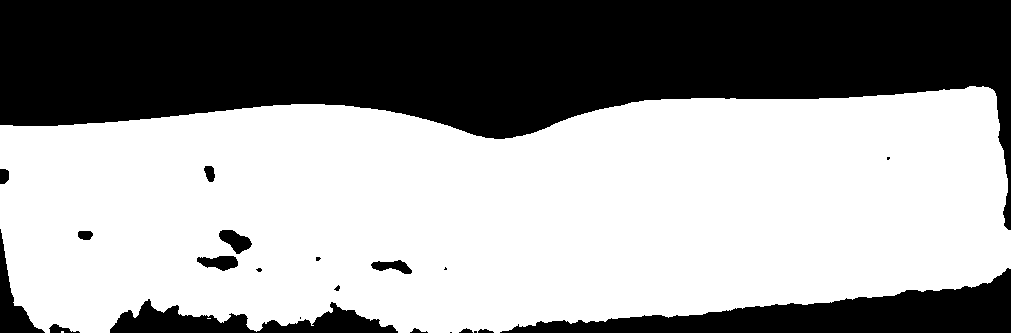
\includegraphics[width=\textwidth]{imagenes/espesor_coroides/Algoritmo_27_fovea_threshold.png}}
      \end{figure}

  \item \textbf{Una vez binarizada la imagen, se procede a hacer un
      ``barrido'' vertical}, de arriba hacia abajo y de izquierda a
    derecha. Para reducir el tiempo de computación, se decidió
    recorrer el eje horizontal de la imagen empezando desde un tercio
    de la anchura y acabando en los dos tercios, una vez se aseguró
    que la \emph{\gls{fovea}} siempre se encontraba en esa zona. \\
    \textbf{ El objetivo de este barrido es el de encontrar}, en cada
    iteración vertical, el primer punto blanco, que se corresponde con
    la línea en la que está \textbf{la \emph{\gls{fovea}}}. Además,
    mientras itera sobre el eje horizontal, busca la posición en el
    que este punto blanco está más abajo.

      \begin{figure}[H]
        \caption{Zona en la que se realiza el barrido}
        \centering \setlength\fboxsep{0pt} \setlength\fboxrule{0.5pt}
        \fbox{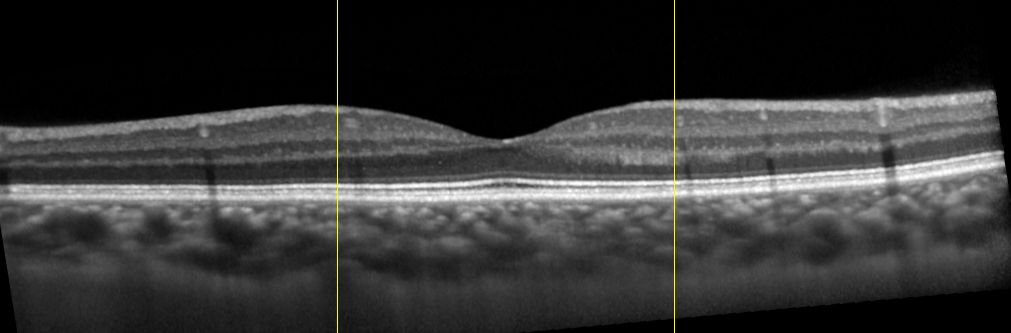
\includegraphics[width=\textwidth]{imagenes/espesor_coroides/Algoritmo_28_fovea_lines.png}}
      \end{figure}

  \item En más de una ocasión surge un pequeño inconveniente que
    proviene de someter la imagen al \emph{threshold binario}: no hay
    un ``punto más bajo'', sino que aparece una línea horizontal en su
    lugar porque el \emph{threshold binario} transforma las curvas en
    escaleras, con muchos ``puntos más bajos'', haciendo que la
    \emph{\gls{fovea}} quedara descentrada. Para resolver esto y tras
    comprobar la simetría de esta línea con respecto a la vertical que
    pasa por la \emph{\gls{fovea}}, en lugar de un único punto, se
    calcularon dos: El primero, el punto de la línea más a la
    izquierda; el segundo, el punto de la línea más a la
    derecha. 

      \begin{figure}[H]
        \caption{Puntos encontrados}
        \centering \setlength\fboxsep{0pt} \setlength\fboxrule{0.5pt}
        \fbox{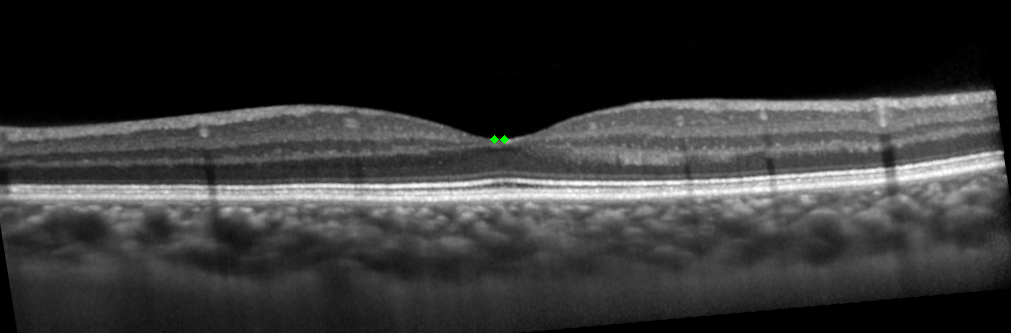
\includegraphics[width=\textwidth]{imagenes/espesor_coroides/Algoritmo_30_fovea_points.png}}
      \end{figure}

  \item Haciendo la media de dichos
    puntos, se encuentra el punto medio: la \emph{\gls{fovea}}. \\
    Nótese que en los casos en que esta línea no se genera y hay un
    único punto ``más bajo'', este algoritmo sigue siendo válido, pues
    el punto más a la derecha y el punto más a la izquierda coinciden,
    y la media de un elemento repetido es el mismo elemento.

      \begin{figure}[H]
        \caption{Punto de la \emph{fóvea}}
        \centering \setlength\fboxsep{0pt} \setlength\fboxrule{0.5pt}
        \fbox{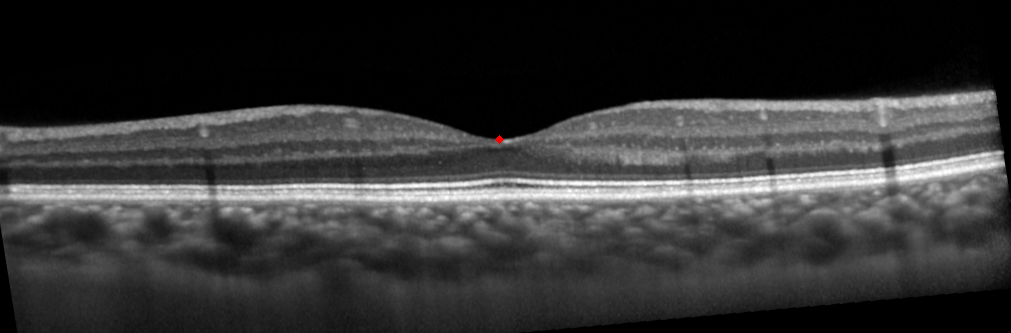
\includegraphics[width=\textwidth]{imagenes/espesor_coroides/Algoritmo_31_fovea_point.png}}
      \end{figure}

  \end{enumerate}
\item \textbf{La última fase se divide en} tres grandes pasos:
  encontrar el punto superior de la \emph{\gls{coroides}} por el que
  pasa la misma vertical que por la \emph{\gls{fovea}}; encontrar el
  punto inferior de la \emph{\gls{coroides}} por el que pasa la misma
  vertical; medir la distancia entre los dos puntos y mostrar el
  resultado en micras.
  \begin{enumerate}[label*=\arabic*.]
  \item \textbf{Primero se determina la posición del punto superior de
      la \emph{\gls{coroides}}} de la siguiente manera:
    \begin{enumerate}[label*=\arabic*.]
    \item Se somete una copia de la imagen horizontal a un
      \emph{threshold binario} con un valor umbral de $179$ y se usa
      un \emph{Canny} para obtener los bordes.
    \item Sobre la imagen resultante se busca en la vertical que pasa
      por la \emph{\gls{fovea}}, de abajo hacia arriba y empezando en
      un cuarto de la altura de la imagen (esto evita fallos
      provocados por una zona negra generada durante la corrección de
      la inclinación), el primer punto negro. Este será el punto
      superior de la \emph{\gls{coroides}}.
    \end{enumerate}
  \item \textbf{Luego se determina la posición del punto inferior de
      la \emph{\gls{coroides}}} de la siguiente manera:
    \begin{enumerate}[label*=\arabic*.]
    \item Como en el paso anterior, se transforma una copia de la
      imagen para calcular el punto. En este ocasión se utiliza
      primero un \emph{median Blur} con un \emph{kernel} de tamaño
      $13$ para eliminar ruido granulado.
    \item Una vez eliminado el ruido, se utiliza un \emph{threshold
        adaptativo
        gaussiano\deftecnica{tecnica:threshold-adaptativo-gauss}} con
      un valor umbral de $173$ para \emph{binarizar} la imagen.
    \item Usando la función
      \emph{findContours\deftecnica{tecnica:contornos}} se genera un
      \emph{Canny\deftecnica{tecnica:canny}} para encontrar los
      bordes, descartando los bordes más pequeños (ruido no eliminado
      por el \emph{Median Blur}).
    \item Una vez eliminado el ruido y detectados los bordes, se busca
      sobre la vertical que pasa por la \emph{\gls{fovea}}, de abajo
      hacia arriba y empezando en los $6/7$ de la altura de la imagen,
      el primer punto blanco, que se corresponde con el borde inferior
      de la \emph{\gls{coroides}} y señala el segundo punto que se
      necesita para medir su espesor.
    \end{enumerate}
  \item \textbf{Una vez determinados los dos puntos que delimitan la
      \gls{coroides} se puede determinar la medida de la misma}.
    \begin{enumerate}[label*=\arabic*.]
    \item Como la imagen está horizontal y los dos puntos encontrados
      se encuentran sobre la misma vertical, la distancia entre ellos
      se puede calcular restando los valores de sus coordenadas sobre
      el eje de ordenadas.
    \item Como esta resta devuelve un resultado en \emph{píxeles}, es
      necesario calcular la relación entre micras y píxeles. Para ello
      se ha usado la proporción indicada en la parte inferior
      izquierda de la imagen original. Se obtuvieron dos proporciones
      diferentes debido a que se encontraron dos imágenes con
      diferente resolución: 1 píxel = 4 micras, y 1 píxel = 6 micras.
    \item Sabiendo la resolución de la imagen, calcular la distancia
      en micras entre los dos puntos es realizar una sencilla
      multiplicación.
    \end{enumerate}
  \end{enumerate}
\end{enumerate}

\subsection{Tiempo de procesamiento}
Aunque se ha tenido un especial cuidado en la elaboración del código;
el tiempo de procesamiento de los algoritmos no ha sido objetivo de
estudio, ni se ha tenido en cuenta en este trabajo. Sí se ha
considerado hacer una evaluación del mismo para futuras
consideraciones y restricciones como tiempo
real y vídeo.\\
Para este proceso se elaboró un ``caso peor'' de $70$ imágenes a
procesar de manera consecutiva, un número muy superior al estudio real
del historial individual de cualquier paciente.\\
\begin{center}
  $70$ imágenes procesadas $\approx$ $43$ segundos
  \\[0.5cm]
  $\frac{43 \text{ segundos}}{70 \text{ imágenes}} \approx 0,614 \text{
    segundos de media por cada imagen}$
\end{center}
Con el resultado calculado de $0,614$ segundos por imagen, sí puede
pensar en aplicar el algoritmo en tiempo real y vídeo. Aunque por
defecto todas las técnicas de las bibliotecas se realizan con
optimizaciones, si se realizase un análisis minucioso del código y su
tiempo de ejecución de las operaciones con menor rendimiento se podría
reducir todavía más el tiempo de procesamiento. Sin embargo, como el
procesamiento de cada imagen es radicalmente inferior al tiempo de
estudio por parte de un oftalmólogo en realizar el mismo proceso, se
descartó completamente un análisis de este tipo y en dar más
relevancia a este apartado.
